\documentclass[spanish,12pt,a4paper]{article}
	\pagestyle{headings}
	\title{\textbf{\Huge{descriptive.mac}\\
                       \large{Un paquete de Maxima para estad\'{\i}stica descriptiva}}}
	\author{\Large{Mario Rodr\'{\i}guez Riotorto}\\
	  \\
	  www.biomates.net\\
	  }
	\setlength{\oddsidemargin}{1cm}
	\setlength{\textwidth}{14cm}
	\setlength{\topmargin}{1.2cm}
	\setlength{\textheight}{20cm}
	\usepackage{graphicx}
	\usepackage{lscape}
	\usepackage[spanish, activeacute]{babel}
	\usepackage{amsfonts}
	\usepackage{latexsym}
	\usepackage{amsmath,amsthm}
	\usepackage{color}\pagecolor{white}

	\newcommand{\normal}{\mathcal{N}}
	\newcommand{\N}{\mathbb{N}}
	\newcommand{\Z}{\mathbb{Z}}
	\newcommand{\Q}{\mathbb{Q}}
	\newcommand{\R}{\mathbb{R}}

% versi'on: 10-06-05

\begin{document}
\maketitle
% \newpage
\tableofcontents

\section{Introducci'on}

El paquete \verb|descriptive.mac| contiene un conjunto de funciones para realizar c'alculos y gr'aficos dentro del 'ambito de la estad'istica descriptiva. Puede descargarse, junto con este documento y datos muestrales (\verb|pidigits.data|, \verb|wind.data| y \verb|biomed.data|), del sitio \emph{www.biomates.net}. Este material se distribuye bajo licencia GPL.

A continuaci'on un ejemplo de c'omo las funciones descriptivas de \verb|descriptive.mac| realizan su cometido, dependiendo de la naturaleza de sus argumentos, listas o matrices,
\begin{verbatim}
(%i1) batchload("descriptive.mac")$
(%i2) /* muestra univariante */
      mean([a,b,c]);
                         c + b + a
(%o2)                    ---------
                             3
(%i3) /* muestra multivariante */
      matrix([a,b],[c,d],[e,f]);
                          [ a  b ]
                          [      ]
(%o3)                     [ c  d ]
                          [      ]
                          [ e  f ]
(%i4) mean(%);
                    e + c + a  f + d + b
(%o4)              [---------, ---------]
                        3          3


\end{verbatim}
N'otese que en las muestras multivariantes la media se calcula para cada columna.

En caso de tener varias muestras con posibles tama~nos muestrales diferentes, la funci'on de Maxima \verb|map| podr'a utilizarse para obtener los resultados deseados de cada muestra,
\begin{verbatim}
(%i5) map(mean,[[a,b,c],[d,e]]);
                      c + b + a  e + d
(%o5)                [---------, -----]
                          3        2
\end{verbatim}
En este caso, se han guardado dos muestras de tama~nos 3 y 2 dentro de una lista.

\section{Entrada de listas y matrices de datos}

Muestras univariantes deben guardarse en listas, tal como se muestra a continuaci'on
\begin{verbatim}
(%i1) s1:[3,1,4,1,5,9,2,6,5,3,5];
(%o1)       [3, 1, 4, 1, 5, 9, 2, 6, 5, 3, 5]
\end{verbatim}
y muestras multivariantes en matrices, como en
\begin{verbatim}
(%i2) s2:matrix([13.17, 9.29],[14.71, 16.88],[18.50, 16.88],
                [10.58,  6.63],[13.33, 13.25],[13.21, 8.12]);
                      [ 13.17  9.29  ]
                      [              ]
                      [ 14.71  16.88 ]
                      [              ]
                      [ 18.5   16.88 ]
(%o2)                 [              ]
                      [ 10.58  6.63  ]
                      [              ]
                      [ 13.33  13.25 ]
                      [              ]
                      [ 13.21  8.12  ]
\end{verbatim}
En este caso, el n'umero de columnas es igual a la dimensi'on de la variable aleatoria y el n'umero de filas al tama~no muestral.

Los datos se pueden introducir manualmente, pero las muestras grandes se suelen guardar en ficheros de texto. Por ejemplo, el fichero \verb|pidigits.data| contiene los 100 primeros d'igitos del n'umero $\pi$:
\begin{verbatim}
      3
      1
      4
      1
      5
      9
      2
      6
      5
      3 ...
\end{verbatim}

Para cargar estos d'igitos en Maxima,
\begin{verbatim}
(%i3) load("numericalio.lisp")$
(%i4) s1:read_list("pidigits.data")$
(%i5) length(s1);
(%o5)                      100
\end{verbatim}

El fichero \verb|wind.data| contiene las velocidades medias del viento registradas diariamente en 5 estaciones meteorol'ogicas en la Rep'ublica de Irlanda\footnote{Este fichero es parte de un conjunto de registros correspondientes a 12 estaciones meteorol'ogicas. El fichero original se puede descargar libremente del StatLib Data Repository y su an'alisis se discute en \cite{hasl}}. Lo que sigue carga los datos,
\begin{verbatim}
(%i6) s2:read_matrix("wind.data")$
(%i7) length(s2);
(%o7)                      100
(%i8) s2[%]; /* ultimo registro */
(%o8)         [3.58, 6.0, 4.58, 7.62, 11.25]
\end{verbatim}

Algunas muestras contienen datos no num'ericos. Como ejemplo, el fichero \verb|biomed.data|\footnote{Este fichero es parte de otro mayor descargado del StatLib Data Repository} contiene cuatro medidas sangu'ineas tomadas en dos grupos de pacientes, \verb|A| y \verb|B|, de edades diferentes,
\begin{verbatim}
(%i9) s3:read_matrix("biomed.data")$
(%i10) length(s3);
(%o10)                      100
(%i11) s3[1]; /* primer registro */
(%o11)        [A, 30, 167.0, 89.0, 25.6, 364]
\end{verbatim}
El primer individuo pertenece al grupo \verb|A|, tiene 30 a~nos de edad y sus cuatro medidas sangu'ineas fueron 167.0, 89.0, 25.6 y 364.

Se debe tener cuidado cuando se trabaja con datos categ'oricos. En el siguiente ejemplo, al s'imbolo \verb|a| se le asigna un valor en alg'un momento anterior y posteriormente se toma una muestra con un valor categ'orico \verb|a|,
\begin{verbatim}
(%i12) a:1$
(%i13) matrix([a,3],[b,5]);
                          [ 1  3 ]
(%o13)                    [      ]
                          [ b  5 ]
\end{verbatim}


\section{Tratamiento de muestras}

Las funciones que se describen en esta secci'on ayudan a extraer alguna informaci'on previa de las muestras o a transformarlas. En primer lugar, puesto que 'esta es una nueva sesi'on de Maxima, se leen las tres muestras nuevamente y se carga el paquete \verb|descriptive.mac|,
\begin{verbatim}
(%i1) load("numericalio.lisp")$
(%i2) s1:read_list("pidigits.data")$
(%i3) s2:read_matrix("wind.data")$
(%i4) s3:read_matrix("biomed.data")$
(%i5) batchload("descriptive.mac")$
\end{verbatim}


\begin{description}

\item[cfrec] El argumento de esta funci'on debe ser una lista de n'umeros, los cuales ser'an posteriormente agrupados en intervalos y se hace el recuento de cu'antos de ellos pertenecen a cada grupo. Alternativamente, la funci'on \verb|cfrec| admite un segundo par'ametro que indica el n'umero de clases, siendo 10 su valor por defecto,
\begin{verbatim}
(%i6) cfrec(s1,5);
(%o6) [[0, 1.8, 3.6, 5.4, 7.2, 9.0], [16, 24, 18, 17, 25]]
\end{verbatim}
La primera lista contiene los l'imites de los intervalos de clase y la segunda los recuentos correspondientes: hay 16 d'igitos dentro del intervalo $[0, 1.8]$, eso es ceros y unos, 24 d'igitos en $(1.8, 3.6]$, es decir, doses y treses, etc.

\item[dfrec] Hace el recuento de las frecuencias absolutas en muestras discretas, tanto num'ericas como categ'oricas. Su 'unico argumento es una lista,
\begin{verbatim}
(%i7) dfrec(s1);
(%o7) [[0, 1, 2, 3, 4, 5, 6, 7, 8, 9],
                        [8, 8, 12, 12, 10, 8, 9, 8, 12, 13]]
(%i8) dfrec(transpose(col(s3,1))[1]);
(%o8)               [[A, B], [35, 65]]
\end{verbatim}
La primera lista devuelve los valores muestrales y la segunda sus frecuencias absolutas. Las instrucciones \verb|? col| y \verb|? transpose| ayudar'an al usuario a comprender la 'ultima entrada.

\item[subsample] En cierto modo esta es una variante de la funci'on \verb|submatrix| de Maxima. El primer argumento es el nombre de la matriz de datos, el segundo es una expresi'on l'ogica sin evaluar (con ap'ostrofo \verb|'|) y adem'as admite opcionalmente argumentos adicionales con los n'umeros de las columnas deseadas. Su comportamiento se entender'a mejor con ejemplos,
\begin{verbatim}
(%i9) subsample(s2,'(%c[1]>18));
           [ 19.38  15.37  15.12  23.09  25.25 ]
           [                                   ]
           [ 18.29  18.66  19.08  26.08  27.63 ]
(%o9)      [                                   ]
           [ 20.25  21.46  19.95  27.71  23.38 ]
           [                                   ]
           [ 18.79  18.96  14.46  26.38  21.84 ]
\end{verbatim}
Estos son los registros multivariantes en los cuales las velocidades del viento en la primera estaci'on meteorol'ogica fueron mayores que 18. V'ease que en la expresi'on l'ogica la $i$-'esima componente es referenciada como \verb|%c[i]|. El s'imbolo \verb|%c| se utiliza dentro de la funci'on \verb|subsample|, raz'on por la cual cuando se utiliza como variable categ'orica podemos confundir a Maxima. En el siguiente ejemplo, pedimos 'unicamente la primera, segunda y quinta componentes de aquellos registros con velocidades del viento mayores o iguales a 16 en la estaci'on n'umero 1 y menores que 25 nudos en la estaci'on n'umero 4,
\begin{verbatim}
(%i10) subsample(s2,'(%c[1]>=16 and %c[4]<25),1,2,5);
                  [ 19.38  15.37  25.25 ]
                  [                     ]
                  [ 17.33  14.67  19.58 ]
(%o10)            [                     ]
                  [ 16.92  13.21  21.21 ]
                  [                     ]
                  [ 17.25  18.46  23.87 ]
\end{verbatim}

Aqu'i un ejemplo con las variables categ'oricas de \verb|biomed.data|. Queremos los registros correspondientes a aquellos pacientes del grupo \verb|B| mayores de 38 a~nos,
\begin{verbatim}
(%i11) subsample(s3,'(%c[1]=B and %c[2]>38));
             [ B  39  28.0  102.3  17.1  146 ]
             [                               ]
             [ B  39  21.0  92.4   10.3  197 ]
             [                               ]
             [ B  39  23.0  111.5  10.0  133 ]
             [                               ]
             [ B  39  26.0  92.6   12.3  196 ]
(%o11)       [                               ]
             [ B  39  25.0  98.7   10.0  174 ]
             [                               ]
             [ B  39  21.0  93.2   5.9   181 ]
             [                               ]
             [ B  39  18.0  95.0   11.3  66  ]
             [                               ]
             [ B  39  39.0  88.5   7.6   168 ]
\end{verbatim}

Probablemente, nuestro an'alisis estad'istico se interesar'a 'unicamente por las mediciones sangu'ineas,
\begin{verbatim}
(%i12) subsample(s3,'(%c[1]=B and %c[2]>38),3,4,5,6);
                 [ 28.0  102.3  17.1  146 ]
                 [                        ]
                 [ 21.0  92.4   10.3  197 ]
                 [                        ]
                 [ 23.0  111.5  10.0  133 ]
                 [                        ]
                 [ 26.0  92.6   12.3  196 ]
(%o12)           [                        ]
                 [ 25.0  98.7   10.0  174 ]
                 [                        ]
                 [ 21.0  93.2   5.9   181 ]
                 [                        ]
                 [ 18.0  95.0   11.3  66  ]
                 [                        ]
                 [ 39.0  88.5   7.6   168 ]
\end{verbatim}

Ahora, calcularemos la media multivariante de \verb|s3|,
\begin{verbatim}
(%i13) mean(s3);
        65 B + 35 A  317          6 NA + 8145.0
(%o13) [-----------, ---, 87.178, -------------, 18.123,
            100      10                100
                                               3 NA + 19587
                                               ------------]
                                                   100
\end{verbatim}
La primera componente del resultado no tiene sentido, ya que \verb|A| y \verb|B| son categ'oricas, la segunda componente es la edad media de los individuos en formato de fracci'on, y el cuarto y 'ultimo valores muestran un comportamiento extra~no. Esto se debe a que el s'imbolo \verb|NA| se utiliza aqu'i para indicar un dato faltante (\emph{non available}) y las dos medias carecen absolutamente de sentido. Una posible soluci'on ser'ia extraer de la muestra aquellas filas con s'imbolos \verb|NA|, aunque tal proceder acarrear'ia p'erdida de informaci'on,
\begin{verbatim}
(%i14) mean(subsample(s3,'(%c[4]#NA and %c[6]#NA),3,4,5,6));
(%o14) [79.4923076923077, 86.2032967032967,
                                                       2514
                                    16.93186813186813, ----]
                                                        13
\end{verbatim}


\end{description}


\section{Estad'istica descriptiva univariante}

Sea $(x_1, x_2, \ldots, x_n)$ una muestra de tama~no $n$. Como ya se ha comentado anteriormente, los datos pueden 
introducirse manualmente o ser le'idos desde un fichero. En los ejemplos siguientes, \verb|s1| guardar'a los 100 primeros d'igitos del n'umero $\pi$ y los c'alculos se har'an en base a ellos.

\begin{verbatim}
(%i1) batchload("descriptive.mac")$
(%i2) load("numericalio.lisp")$
(%i3) s1:read_list("pidigits.data")$
\end{verbatim}


\begin{description}

\item[mean] Esta es la media muestral, definida como
\[
\bar{x}=\frac{1}{n} \sum_{i=1}^n x_i.
\]
\begin{verbatim}
(%i4) mean(s1);
                            471
(%o4)                       ---
                            100
(%i5) numer:true$   %o4;
(%o5)                      4.71
\end{verbatim}
De ahora en adelante, todos los resultados se dar'an en notaci'on decimal.

\item[var, var1] Hay dos alternativas para la varianza muestral. La funci'on \verb|var| calcula
\[
s^2=\frac{1}{n} \sum_{i=1}^n (x_i-\bar{x})^2,
\]
dividiendo entre $n$, y \verb|var1| devuelve
\[
s_1^2=\frac{n}{n-1}s^2.
\]
\begin{verbatim}
(%i6) var(s1);
(%o6)               8.425899999999999
(%i7) var1(s1);
(%o7)                8.5110101010101
\end{verbatim}

\item[std, std1] La funci'on \verb|std| es la ra'iz cuadrada de $s^2$,
\[
s=\sqrt{\frac{1}{n} \sum_{i=1}^n (x_i-\bar{x})^2},
\]
y \verb|std1| se obtiene de $s_1^2$
\[
s_1=\sqrt{\frac{n}{n-1}s^2}.
\]
\begin{verbatim}
(%i8) std(s1);
(%o8)               2.902740084816414
(%i9) std1(s1);
(%o9)               2.917363553109228
\end{verbatim}

\item[ncmoment, cmoment] El momento no central de orden $k$ se define como
\[
a_k=\frac{1}{n} \sum_{i=1}^n x_i^k
\]
\begin{verbatim}
(%i10) ncmoment(s1,1); /* la media */
(%o10)                      4.71
\end{verbatim}

El momento central de orden $k$ es
\[
m_k=\frac{1}{n} \sum_{i=1}^n (x_i - \bar{x})^k
\]
y se calcula como
\begin{verbatim}
(%i11) cmoment(s1,2); /* the variance */
(%o11)               8.425899999999999
\end{verbatim}

\item[vc] El coeficiente de variaci'on es el cociente entre la desviaci'on t'ipica est'andar muestral y la media,
\[
\mbox{V}= \frac{s_1}{\bar{x}}.
\]
\begin{verbatim}
(%i12) vc(s1);
(%o12)               .6193977819764815
\end{verbatim}

\item[mini, maxi] Estos son los valores extremos de la muestra, el m'inimo
\[
x_{(1)}=\min\{x_i: 1 \leq i \leq n\},
\]
y el m'aximo
\[
x_{(n)}=\max\{x_i: 1 \leq i \leq n\}.
\]
\begin{verbatim}
(%i13) [mini(s1), maxi(s1)];
(%o13)                     [0, 9]
\end{verbatim}

\item[range] El rango es la diferencia entre los valores extremos, $\mbox{range}=x_{(1)}-x_{(n)}$.
\begin{verbatim}
(%i14) range(s1);
(%o14)                       9
\end{verbatim}

\item[median] Una vez ordenada la muestra, la mediana es el valor central,
\[
\mbox{med}= \left\{ \begin{array}{ll}
               \frac{1}{2} (x_{\frac{n}{2}} + x_{\frac{n}{2} + 1}) & \mbox{si $n$ es par} \\
               x_{\frac{n+1}{2}}                               & \mbox{si $n$ es impar}
            \end{array} \right.
\]
\begin{verbatim}
(%i15) median(s1);
(%o15)                      4.5
\end{verbatim}

\item[quantile] Aunque hay varias definiciones del cuantil muestral \cite{hynd}, la que se basa en la interpolaci'on lineal es la que est'a programada en \verb|descriptive.mac|. Sea $(x_{(1)}, x_{(2)}, \ldots, x_{(n)})$ la muestra ordenada, entonces el $p$-cuantil, con $p \in [0,1]$, se define como
\[
c_p= \left\{ \begin{array}{ll}
               x_{(i)} & \mbox{if $i=p n$} \\
               (p n-i)x_{(i+1)}-(p n-i-1)x_{(i)}   & \mbox{if $i < p n <i+1$}
            \end{array} \right.
\]
\begin{verbatim}
(%i16) /* 1er y 3er cuartiles */
       [quantile(s1,1/4),quantile(s1,3/4)];
(%o16)                  [2.0, 7.25]
\end{verbatim}

\item[qrange] El rango intercuart'ilico es la diferencia entre el tercer y primer cuartiles, $c_{3/4}-c_{1/4}$,
\begin{verbatim}
(%i17) qrange(s1);
(%o17)                      5.25
\end{verbatim}

\item[meandev, mediandev] La desviaci'on media y la desviaci'on mediana son
\[
\mbox{MD}= \frac{1}{n} \sum_{i=1}^n |x_i-\bar{x}|
\]
y
\[
\mbox{MedD}=\mbox{med}(|x_i-\mbox{med}(x_i)|),
\]
respectivamente.
\begin{verbatim}
(%i18) meandev(s1);
(%o18)               2.550000000000001
(%i19) mediandev(s1);
(%o19)                      2.5
\end{verbatim}

\item[harmean, geomean] La media arm'onica se define como
\[
\mbox{H} = \frac{n}{\sum_{i=1}^n \frac{1}{x_i}}
\]
y la media geom'etrica como
\[
\mbox{G} = \sqrt[n]{\prod_{i=1}^n x_i}.
\]
Puesto que el cero aparece varias veces en la variable \verb|s1|, \verb|harmean| dar'a un mensaje de error y \verb|geomean| dar'a cero. Por ello en el siguiente ejemplo se evita utilizar \verb|s1| y se define una nueva variable \verb|y|.
\begin{verbatim}
(%i20) y:[5,7,2,5,9,5,6,4,9,2,4,2,5]$
(%i21) [harmean(y),geomean(y)];
(%o21)     [3.901858027632205, 4.454845412337012]
\end{verbatim}

\item[kurtosis] El coeficiente de curtosis se define como
\[
\mbox{Ku}=\frac{\frac{1}{n} \sum_{i=1}^n (x_i-\bar{x})^4}{s^4} -3.
\]
\begin{verbatim}
(%i22) kurtosis(s1);

(%o22)               - 1.219988843897832
\end{verbatim}


\item[skewness] El coeficiente de asimetr'ia se define como
\[
\mbox{Sk}=\frac{\frac{1}{n} \sum_{i=1}^n (x_i-\bar{x})^3}{s^3}.
\]
\begin{verbatim}
(%i23) kurtosis(s1);
(%o23)              - 1.273247946514421
\end{verbatim}

\item[pearskewness, quarskewness] El coeficiente de asimetr'ia de Pearson y el coeficiente de asimetr'ia cuart'ilico se definen como 
\[
\mbox{PSk}= \frac{3 (\bar{x}-\mbox{med}(x_i))}{s}
\]
y
\[
\mbox{QSk}= \frac{c_{3/4}-2 c_{1/2}+c_{1/4}}{c_{3/4}-c_{1/4}},
\]
respectivamente.
\begin{verbatim}
(%i24) pearskewness(s1);
(%o24)               .2159484029093895
(%i25) quarskewness(s1);
(%o25)               .0476190476190476
\end{verbatim}

\end{description}


\section{Estad'istica descriptiva multivariante}


A partir de ahora, sea la matriz
\[
\left(
\begin{array}{cccc}
x_{11}  &  x_{12}  &  \cdots  &  x_{1d}  \\
x_{21}  &  x_{22}  &  \cdots  &  x_{2d}  \\
\vdots  &  \vdots  &          &  \vdots  \\
x_{n1}  &  x_{n2}  &  \cdots  &  x_{nd}
\end{array}
\right)
\]
una muestra de dimensi'on $d$ de tama~no $n$ y
\[
X_i =
\left(
\begin{array}{c}
x_{i1}  \\  x_{i2}  \\  \vdots  \\  x_{id}
\end{array}
\right) = (x_{i1}, x_{i2}, \ldots, x_{id})'
\]
el vector de valores observados en la $i$-'esima unidad muestral. Con esta notaci'on, el vector de medias es
\[
\bar{X} = \frac{X_1 + X_2 + \ldots +X_n}{n}.
\]

Las funciones que se han definido hasta aqu'i se aplican tambi'en a matrices, en cuyo caso se obtendr'an como respuestas vectores de longitud igual a la dimensi'on de la variable estad'istica. En los siguientes ejemplos los c'alculos se realizar'an con las velocidades medias del viento medidas en las cinco estaciones meteorol'ogicas,
\begin{verbatim}
(%i1) batchload("descriptive.mac")$
(%i2) load("numericalio.lisp")$
(%i3) s2:read_matrix("wind.data")$
(%i4) length(s2);  /* tama~no muestral */
(%o4)                       100
(%i5) mean(s2);  /* vector de medias */
(%o5)  [9.9485, 10.1607, 10.8685, 15.7166, 14.8441]
(%i6) var(s2);  /* varianzas */
(%o6) [17.22190675000001, 14.98773651, 15.47572875,
                32.17651044000001, 24.42307619000001]
(%i7) maxi(s2);  /* velocidades medias maximas */
(%o7)      [20.25, 21.46, 20.04, 29.63, 27.63]
(%i8) kurtosis(s2);
(%o8) [- .2715445622195385, 0.119998784429451,
       - .4275233490482866, - .6405361979019522,
       - .4952382132352935]
\end{verbatim}

Un aspecto crucial en el an'alisis estad'istico multivariante es la dependencia estoc'astica entre variables \cite{john,pena}. Medidas de dependencia son las covarianzas y las correlaciones.

\begin{description}

\item[cov, cov1] Hay dos alternativas para la matriz de covarianzas, \verb|cov| calcula
\[
S = \frac{1}{n} \sum_{i=1}^n X_i X_i' - \bar{X} \bar{X}'
\]
y \verb|cov1| eval'ua
\[
S_1  =  \frac{n}{n-1}S 
     =    \left(
          \begin{array}{cccc}
          s_{11}  &  s_{12}  &  \cdots  &  s_{1d}  \\
          s_{21}  &  s_{22}  &  \cdots  &  s_{2d}  \\
          \vdots  &  \vdots  &          &  \vdots  \\
          s_{d1}  &  s_{d2}  &  \cdots  &  s_{dd}
          \end{array}
          \right),
\]
donde $s_{ij}$ es la covarianza muestral entre las componentes aleatorias $X_i$ y $X_j$, y los elementos de la diagonal $s_{ii}$ son las varianzas muestrales.

\begin{verbatim}
(%i9) fpprec:7$ /* cambia precision para mejorar salida */
(%i10) cov(s2);
       [ 17.22191  13.61811  14.37217  19.39624  15.42162 ]
       [                                                  ]
       [ 13.61811  14.98774  13.30448  15.15834  14.9711  ]
       [                                                  ]
(%o10) [ 14.37217  13.30448  15.47573  17.32544  16.18171 ]
       [                                                  ]
       [ 19.39624  15.15834  17.32544  32.17651  20.44685 ]
       [                                                  ]
       [ 15.42162  14.9711   16.18171  20.44685  24.42308 ]
(%i11) cov1(s2);
       [ 17.39587  13.75567  14.51734  19.59216  15.5774  ]
       [                                                  ]
       [ 13.75567  15.13913  13.43887  15.31145  15.12232 ]
       [                                                  ]
(%o11) [ 14.51734  13.43887  15.63205  17.50044  16.34516 ]
       [                                                  ]
       [ 19.59216  15.31145  17.50044  32.50153  20.65338 ]
       [                                                  ]
       [ 15.5774   15.12232  16.34516  20.65338  24.66977 ]
\end{verbatim}


\item[listvar] Esta funci'on devuelve una lista de medidas globales de variaci'on:
\begin{enumerate}
\item \emph{varianza total}: $V_T=\mbox{tr}(S_1)=\sum_{i=1}^d s_{ii}$,
\item \emph{varianza media}: $V_M=\frac{\mbox{tr}(S_1)}{d}$,
\item \emph{varianza generalizada}: $V_G=|S_1|$,
\item \emph{desviaci'on t'ipica generalizada}: $d_G=\sqrt{|S_1|}$,
\item \emph{varianza efectiva} \cite{pena}: $V_E=|S_1|^\frac{1}{p}$,
\item \emph{desviaci'on t'ipica efectiva}: $d_E=|S_1|^\frac{1}{2p}$.
\end{enumerate}
\begin{verbatim}
(%i12) listvar(s2);
(%o12) [105.3383, 21.06767, 12874.35, 113.4652, 6.636591,
                                                   2.576158]
\end{verbatim}

La funci'on \verb|listvar| tiene un argumento l'ogico opcional: \verb|listvar(x,true)| le dice a Maxima que \verb|x| es la matriz de datos, haciendo entonces lo mismo que \verb|listvar(x)|. Por otro lado, \verb|listvar(x,false)| significa que \verb|x| no es la matriz de datos, sino la matriz de covarianzas, evitando calcularla nuevamente,
\begin{verbatim}
(%i13) listvar(%o11,false);
(%o13) [105.3383, 21.06767, 12874.35, 113.4652, 6.636591,
                                                   2.576158]
\end{verbatim}


\item[cor] La matriz de correlaciones se define como $R=\{r_{ij}\}_{i,j = 1, 2, \ldots, d}$, con
\[
r_{ij}=\frac{s_{ij}}{\sqrt{s_{ii} s_{jj}}}.
\]
\begin{verbatim}
(%i14) cor(s2);
       [   1.0     .8476339  .8803515  .8239624  .7519506 ]
       [                                                  ]
       [ .8476339    1.0     .8735834  .6902622  0.782502 ]
       [                                                  ]
(%o14) [ .8803515  .8735834    1.0     .7764065  .8323358 ]
       [                                                  ]
       [ .8239624  .6902622  .7764065    1.0     .7293848 ]
       [                                                  ]
       [ .7519506  0.782502  .8323358  .7293848    1.0    ]
\end{verbatim}

La funci'on \verb|cor| tiene un argumento l'ogico opcional: \verb|cor(x,true)| le dice a Maxima que \verb|x| es la matriz de datos, haciendo entonces lo mismo que \verb|cor(x)|. Por otro lado, \verb|cor(x,false)| significa que \verb|x| no es la matriz de datos, sino la matriz de covarianzas, evitando calcularla nuevamente,
\begin{verbatim}
(%i15) cor(%o11,false); /* mas rapido */
       [   1.0     .8476339  .8803515  .8239624  .7519506 ]
       [                                                  ]
       [ .8476339    1.0     .8735834  .6902622  0.782502 ]
       [                                                  ]
(%o15) [ .8803515  .8735834    1.0     .7764065  .8323358 ]
       [                                                  ]
       [ .8239624  .6902622  .7764065    1.0     .7293848 ]
       [                                                  ]
       [ .7519506  0.782502  .8323358  .7293848    1.0    ]
\end{verbatim}

\item[listdep] Esta funci'on devuelve una lista de medidas de correlaci'on:
\begin{enumerate}
\item \emph{matriz de precisi'on}: $S_1^{-1}=\{s^{ij}\}_{i,j = 1, 2, \ldots, d}$, inversa de la matriz de covarianzas,
\item \emph{vector de correlaciones m'ultiples}: $(R_1^2, R_2^2, \ldots, R_d^2)$, con $R_i^2=1-\frac{1}{s^{ii}s_{ii}}$ siendo un indicador de la bondad de ajuste del modelo de regresi'on lineal multivariante sobre $X_i$ cuando el resto de variables se utilizan como regresores.
\item \emph{matriz de correlaciones parciales}: siendo su elemento $(i, j)$ 
\[
r_{ij.\mbox{rest}}=-\frac{s^{ij}}{\sqrt{s^{ii} s^{jj}}}.
\]
\end{enumerate}
\begin{verbatim}
(%i16) z:listdep(s2)$
(%i17) fpprec:5$ /* para mejorar la salida */
(%i18) z[1];  /* matriz de precision */
       [  .38486   - .13856  - .15626  - .10239   .03118  ]
       [                                                  ]
       [ - .13856   .34107   - .15233   .03845   - .05284 ]
       [                                                  ]
(%o18) [ - .15626  - .15233   .47296   - .02482  - .10054 ]
       [                                                  ]
       [ - .10239   .03845   - .02482   .10937   - .03403 ]
       [                                                  ]
       [  .03118   - .05284  - .10054  - .03403   .14834  ]
(%i19) z[2];  /* vector de correlaciones multiples */
(%o19)    [.85063, .80634, .86474, .71867, .72675]
(%i20) z[3];  /* matriz de correlaciones parciales */
       [  - 1.0     .38244   .36627   .49908   - .13049 ]
       [                                                ]
       [  .38244    - 1.0    .37927  - .19907   .23492  ]
       [                                                ]
(%o20) [  .36627    .37927   - 1.0    .10911    .37956  ]
       [                                                ]
       [  .49908   - .19907  .10911   - 1.0     .26719  ]
       [                                                ]
       [ - .13049   .23492   .37956   .26719    - 1.0   ]
\end{verbatim}

La funci'on \verb|listdep| tiene un argumento l'ogico opcional: \verb|listdep(x,true)| le dice a Maxima que \verb|x| es la matriz de datos, haciendo entonces lo mismo que \verb|listdep(x)|. Por otro lado, \verb|listdep(x,false)| significa que \verb|x| no es la matriz de datos, sino la matriz de covarianzas, evitando calcularla nuevamente.

\end{description}


\section{Gr'aficos estad'isticos}

Hay cuatro tipos de diagramas en \verb|descriptive.mac|. La funci'on \verb|dataplot| permite la visualizaci'on directa de los datos muestrales, \verb|histogram| se relaciona con el an'alisis de los patrones de las frecuencias en caso de observaciones continuas, \verb|barsplot| con las frecuencias de datos categ'oricos o discretos y \verb|boxplot| permite estudiar la propiedad homoced'astica entre muestras. Todas estas funciones necesitan del programa de representaci'on gr'afica \verb|gnuplot|.

Como en anteriores secciones, los d'igitos de $\pi$, las velocidades del viento y las medidas sangu'ineas ser'an utilizadas en los ejemplos,
\begin{verbatim}
(%i1) batchload("descriptive.mac")$
(%i2) load("numericalio.lisp")$
(%i3) s1:read_list("pidigits.data")$
(%i4) s2:read_matrix("wind.data")$
(%i5) s3:read_matrix("biomed.data")$
\end{verbatim}

Las funciones de representaci'on gr'afica se describen a continuaci'on..

\begin{description}

\item[dataplot(data, options)] El argumento \verb|data| debe ser una lista num'erica o una matriz, y con las opciones de \verb|options| se podr'an controlar algunos aspectos del gr'afico por parte del usuario:

\begin{enumerate}
\item \verb|'outpudev|, por defecto \verb|"x"|, indica el dispositivo de salida; valores aceptados son \verb|"x"|, \verb|"eps"| y \verb|"png"|, para la pantalla y los formatos postscript y png, respectivamente.
\item \verb|'maintitle|, por defecto \verb|""|, es el t'itulo principal entre comillas dobles.
\item \verb|'axisnames|, por defecto \verb|["x","y","z"]|, es una lista con los nombres para los ejes $x$, $y$ y $z$.
\item \verb|'joined|, por defecto \verb|false|, un valor l'ogico para seleccionar si los puntos en 2D se quieren unidos por segmentos o aislados.
\item \verb|'picturescales|, por defecto \verb|[1.0, 1.0]|, factores de escala para el tama~no del gr'afico.
\item \verb|'threedim|, por defecto \verb|true|, le dice a Maxima si debe representar una matriz de tres columnas en un diagrama 3D o en un gr'afico de dispersi'on multivariante. Ver ejemplos m'as abajo.
\item \verb|'axisrot|, por defecto \verb|[60, 30]|, cambia el punto de vista cuando \verb|'threedim| tiene asignado el valor \verb|true| y los datos est'an almacenados en una matriz de tres columnas. El primer n'umero es el 'angulo de rotaci'on del eje $x$, y el segundo el 'angulo de rotaci'on del eje $z$, ambos medidos en grados.
\item \verb|'nclasses|, por defecto \verb|10|, es el n'umero de clases para los histogramas en la diagonal de los gr'aficos de dispersi'on multivariantes.
\item \verb|'pointstyle|, por defecto \verb|0|, es un entero para indicar c'omo representar los puntos muestrales.
\end{enumerate}

Por ejemplo, con la siguiente entrada se pide un gr'afico de los primeros veinte d'igitos de $pi$ y la salida se guarda en un fichero eps\footnote{En este documento, los gr'aficos se generan en formato eps.}. El resultado se puede ver en el apartado \emph{a)} de la Figura~\ref{fig1}.
\begin{verbatim}
(%i6) dataplot(makelist(s1[k],k,1,20),
               'outputdev="eps",'pointstyle=3)$
\end{verbatim}
N'otese que que los datos unidimensionales se representan como series cronol'ogicas. En el siguiente caso, con algunos datos m'as y diferentes ajustes,
\begin{verbatim}
(%i7) dataplot(makelist(s1[k],k,1,50),
             'maintitle="First pi digits",
             'axisnames=["digit order","digit value"],
             'pointstyle=1,
             'joined=true,
             'outputdev="eps")$
\end{verbatim}
El resultado se muestra en el apartado \emph{b)} de la Figura~\ref{fig1}.


\begin{figure}
\begin{center}
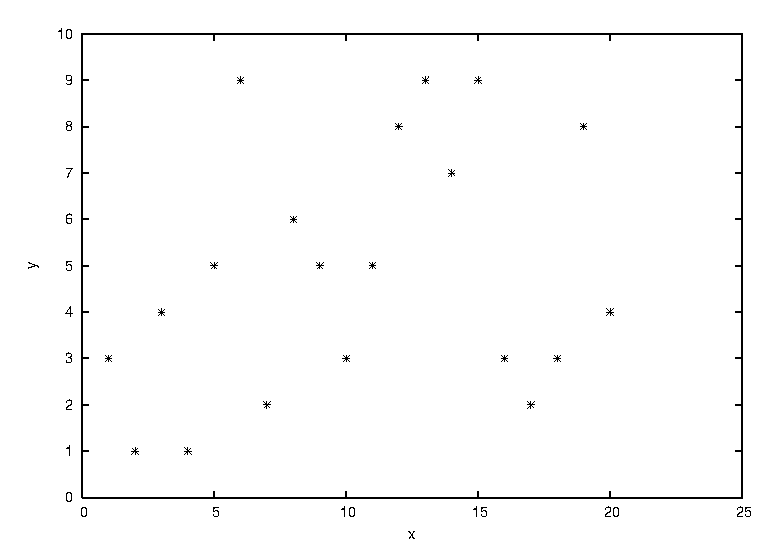
\includegraphics[scale=1.0]{dataplot1.eps} \\
\emph{a)} \\ 
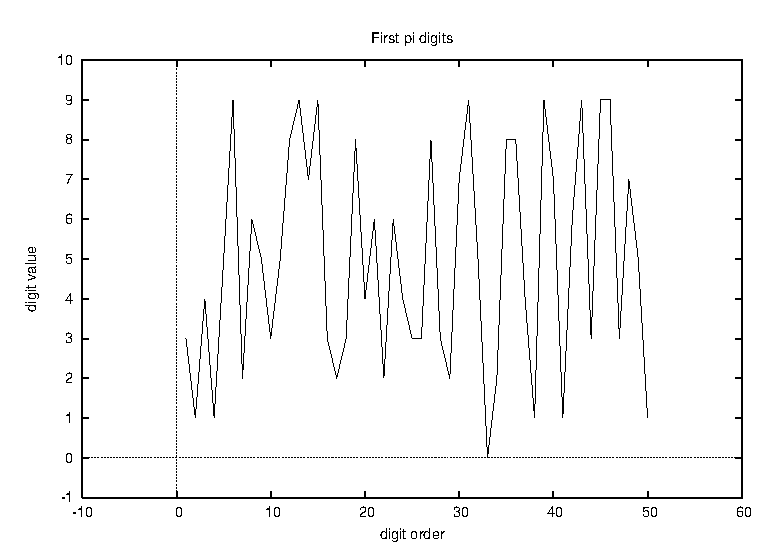
\includegraphics[scale=1.0]{dataplot2.eps} \\
\emph{b)} \\
\caption{Representando muestras univariantes: \emph{a)} puntos aislados; \emph{b)} puntos unidos.}
\label{fig1}
\end{center}
\end{figure}

La funci'on \verb|dataplot| puede usarse para dibujar puntos bidimensionales. El siguiente ejemplo es un gr'afico de dispersi'on de los pares de velocidades del viento correspondientes a la primera y quinta estaciones meteorol'ogicas,
\begin{verbatim}
(%i8) dataplot(submatrix(s2,2,3,4),
         'outputdev="eps", 'pointstyle=1,
         'maintitle="Pairs of wind speeds measured in knots",
         'axisnames=["Wind speed in A","Wind speed in E"])$
\end{verbatim}
La salida en el apartado \emph{a)} de la Figura~\ref{fig2}

Si los puntos se almacenan en una matriz de dos columnas, \verb|dataplot| los puede representar directamente, pero si est'an formateados como una lista de pares, se deben pasar a formato matricial, como en el siguiente ejemplo. El resultado est'a en el apartado \emph{b)} de la Figura~\ref{fig2}
\begin{verbatim}
(%i9) bs:[[64,-104], [64,-99], [61,-95], [57,-95], [55,-94],
          [55,-90], [72,-89], [80,-88], [77,-86], [80,-88], 
          [82,-91], [80,-88], [72,-89], [55,-90], [47,-89], 
          [39,-87], [33,-84], [32,-81], [35,-75], [36,-69], 
          [42,-69], [45,-68], [42,-69], [36,-69], [35,-67], 
          [35,-62], [35,-60], [39,-60], [45,-61], [51,-61], 
          [53,-65], [56,-68], [61,-70], [67,-71], [73,-70], 
          [78,-67], [80,-64], [81,-61], [78,-58], [75,-60], 
          [75,-62], [78,-62], [81,-61], [81,-56], [79,-50], 
          [75,-47], [70,-44], [62,-44], [58,-45], [53,-50], 
          [52,-52], [49,-53], [48,-52], [48,-50], [49,-48], 
          [51,-49], [52,-52], [51,-54], [51,-57], [51,-61], 
          [45,-61], [39,-60], [35,-60], [32,-57], [32,-52], 
          [32,-49], [35,-45], [39,-42], [43,-41], [48,-42], 
          [51,-43], [55,-47], [51,-43], [48,-42], [43,-41], 
          [44,-38], [47,-35], [54,-16], [56,-5], [60,-11], 
          [64,-6], [67,-12], [72,-7], [74,-14], [80,-9], 
          [80,-16], [86,-11], [87,-17], [92,-12], [93,-21], 
          [99,-16], [100,-22], [106,-19], [107,-27], [115,-25], 
          [110,-32], [94,-72], [91,-72], [88,-73], [87,-74], 
          [88,-76], [91,-76], [91,-79], [89,-81], [91,-79], 
          [91,-76], [94,-77], [94,-79], [94,-77], [91,-76], 
          [88,-76], [87,-74], [88,-73], [91,-72], [94,-72], 
          [97,-75], [98,-80], [97,-82], [94,-84], [91,-85], 
          [87,-83], [84,-80], [87,-83], [91,-85], [91,-95], 
          [92,-102], [85,-105], [69,-106], [64,-104]]$
(%i10) dataplot(apply('matrix,bs),
           'outputdev="eps",
           'maintitle="Bart", 'joined=true,
           'axisnames=["","",""],
           'picturescales=[0.5, 1.0])$
\end{verbatim}


\begin{figure}
\begin{center}
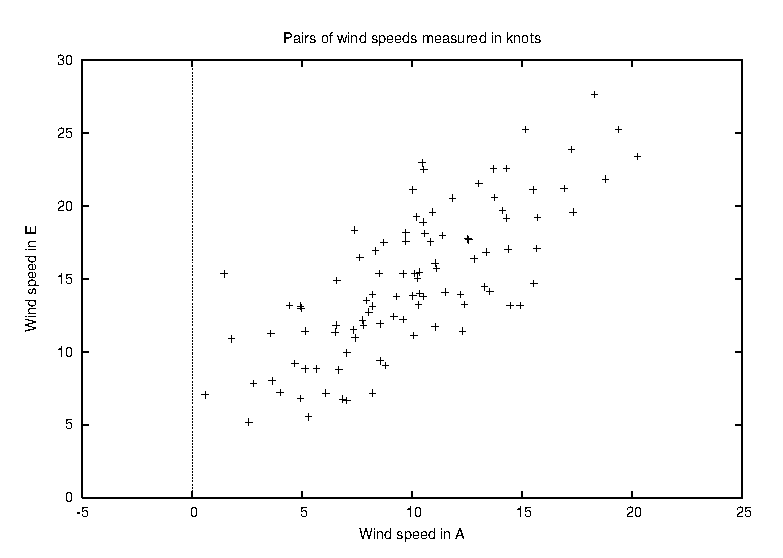
\includegraphics[scale=1.0]{dataplot3.eps} \\
\emph{a)} \\ 
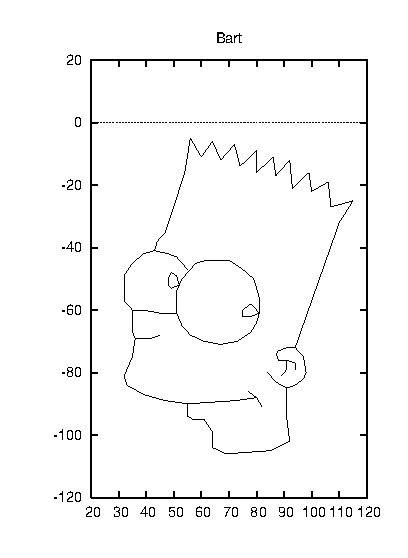
\includegraphics[scale=1.0]{dataplot4.eps} \\
\emph{b)} \\
\caption{Representando muestras bivariantes: \emph{a)} diagrama de dispersi'on; \emph{b)} puntos unidos.}
\label{fig2}
\end{center}
\end{figure}

Nubes de puntos en tres dimensiones se pueden ver como una proyecci'on en el plano. En  este ejemplo, son solicitados gr'aficos de las velocidades del viento correspondientes a tres estaciones meteorol'ogicas, primero en tres dimensiones y luego en un diagrama de dispersi'on multivariante \cite{john}, 
\begin{verbatim}
(%i11) /* Grafico 3D */
       dataplot(submatrix(s2,4,5), 'pointstyle=2,
         'outputdev="eps", 'picturescales=[0.6, 0.6],
         'maintitle="Pairs of wind speeds measured in knots",
         'axisnames=["Station A","Station B","Station C"])$
(%i12) /* Grafico dispersion multivariante */
       dataplot(submatrix(s2,4,5),
         'outputdev="eps", 'nclasses=6, 'threedim=false)$
\end{verbatim}
Se observar'a que en el 'ultimo ejemplo el n'umero de clases en los histogramas de la diagonal se ajusta a 6 y que a la opci'on \verb|'threedim| se le da el valor \verb|false|. Ambos diagramas est'an en la Figura~\ref{fig3}.


\begin{figure}
\begin{center}
\includegraphics[scale=1.0,angle=270]{dataplot5.eps} \\
\emph{a)} \\ 
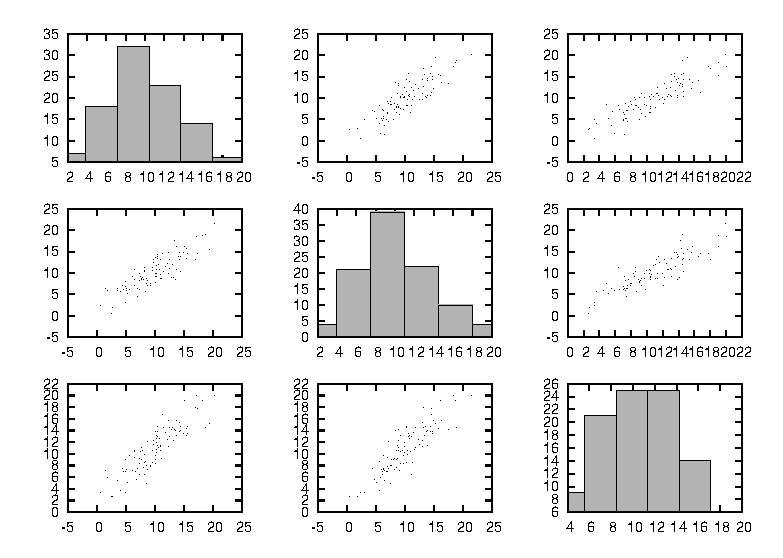
\includegraphics[scale=1.0]{dataplot6.eps} \\
\emph{b)} \\
\caption{Muestras tridimensionales: \emph{a)} 3D; \emph{b)} dispersi'on multivariante.}
\label{fig3}
\end{center}
\end{figure}

Para m'as de tres dimensiones s'olo son posibles los diagramas de dispersi'on multivariantes, como en
\begin{verbatim}
(%i13) dataplot(s2,'outputdev="eps")$
\end{verbatim}


\item[histogram(data, options)] Esta funci'on dibuja un histograma. Los datos en \verb|data| deben almacenarse en una lista de n'umeros o en una matriz de una columna. Tambi'en aqu'i hay algunas opciones,

\begin{enumerate}
\item \verb|'outpudev|, por defecto \verb|"x"|, indica el dispositivo de salida; valores aceptados son \verb|"x"|, \verb|"eps"| y \verb|"png"|, para la pantalla y los formatos postscript y png, respectivamente.
\item \verb|'maintitle|, por defecto \verb|""|, es el t'itulo principal entre comillas dobles.
\item \verb|'axisnames|, por defecto \verb|["x", "Fr."]|, es una lista con los nombres para los ejes $x$ e $y$.
\item \verb|'picturescales|, por defecto \verb|[1.0, 1.0]|, factores de escala para el tama~no del gr'afico.
\item \verb|'nclasses|, por defecto \verb|10|, es el n'umero de clases o barras.
\item \verb|'relbarwidth|, por defecto \verb|0.9|, un n'umero decimal entre 0 y 1 para controlar el ancho de las barras.
\item \verb|'barcolor|, por defecto \verb|1|, un entero para indicar el color de las barras.
\item \verb|'colorintensity|, por defecto \verb|1|, un n'umero decimal entre 0 y 1 para fijar la intensidad del color.
\end{enumerate}

En los pr'oximos dos ejemplos se solicitan histogramas para los primeros 100 d'igitos del n'umero $\pi$ y para las velocidades del viento en la tercera estaci'on meteorol'ogica. Los dos histogramas est'an reproducidos en la Figura~\ref{fig4}.
\begin{verbatim}
(%i14) histogram(s1,'maintitle="pi digits",
                 'axisnames=["","Absolute frequency"],
                 'relbarwidth=0.2,'barcolor=3,
                 'colorintensity=0.6,'outputdev="eps")$
(%i15) histogram(col(s2,3),
                 'outputdev="eps",'colorintensity=0.3)$
\end{verbatim}
En el primer caso, \verb|s1| es una lista y en el segundo ejemplo, \verb|col(s2,3)| es una matriz.

\begin{figure}
\begin{center}
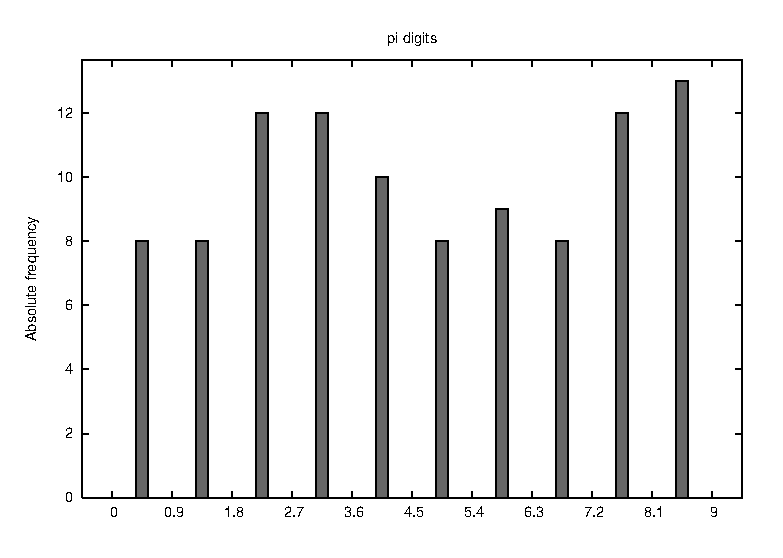
\includegraphics[scale=1.0]{histogram1.eps} \\
\emph{a)} \\ 
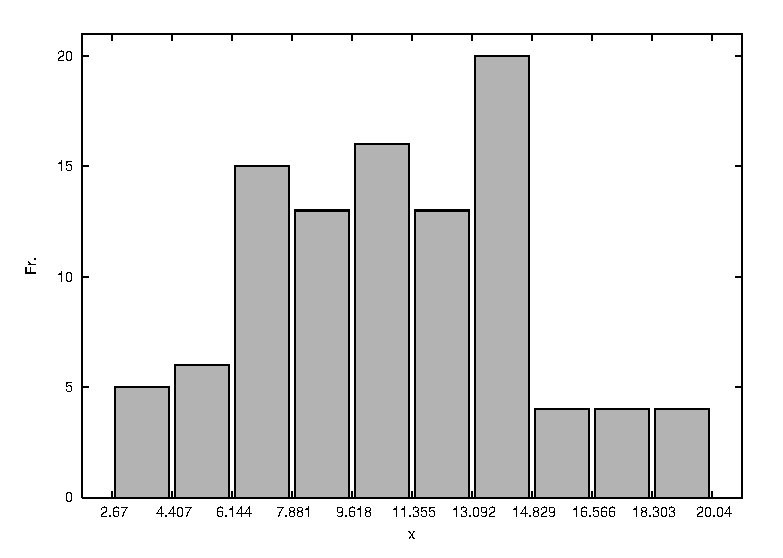
\includegraphics[scale=1.0]{histogram2.eps} \\
\emph{b)} \\
\caption{Histogramas: \emph{a)} d'igitos de $\pi$; \emph{b)} velocidades del viento.}
\label{fig4}
\end{center}
\end{figure}

\item[barsplot(data, options)] Como los histogramas pero para variables estad'isticas discretas, num'ericas o categ'oricas.

\begin{enumerate}
\item \verb|'outpudev|, por defecto \verb|"x"|, indica el dispositivo de salida; valores aceptados son \verb|"x"|, \verb|"eps"| y \verb|"png"|, para la pantalla y los formatos postscript y png, respectivamente.
\item \verb|'maintitle|, por defecto \verb|""|, es el t'itulo principal entre comillas dobles.
\item \verb|'axisnames|, por defecto \verb|["x", "Fr."]|, es una lista con los nombres para los ejes $x$ e $y$.
\item \verb|'picturescales|, por defecto \verb|[1.0, 1.0]|, factores de escala para el tama~no del gr'afico.
\item \verb|'relbarwidth|, por defecto \verb|0.9|, un n'umero decimal entre 0 y 1 para controlar el ancho de las barras.
\item \verb|'barcolor|, por defecto \verb|1|, un entero para indicar el color de las barras.
\item \verb|'colorintensity|, por defecto \verb|1|, un n'umero decimal entre 0 y 1 para fijar la intensidad del color.
\end{enumerate}

En primer lugar, obtengamos el gr'afico de barras para los grupos \verb|A| y \verb|B| de pacientes en la muestra \verb|s3|,
\begin{verbatim}
(%i17) barsplot(col(s3,1),
         'outputdev="eps",
         'maintitle="Groups of patients",
         'axisnames=["Group","# of individuals"],
         'colorintensity=0.2)$
\end{verbatim}
Recu'erdese que la primera columna de la muestra \verb|s3| guarda los valores categ'oricos \verb|A| y \verb|B|, tambi'en llamados en ocasiones factores. Por otro lado, los n'umeros enteros positivos en la segunda columna son las edades, en a~nos, que es una variable discreta, por lo que podemos representar las frecuencias absolutas para estos valores,
\begin{verbatim}
(%i18) barsplot(col(s3,2),
         'outputdev="eps",
         'maintitle="Ages",
         'axisnames=["Years","# of individuals"],
         'colorintensity=0.2,
         'relbarwidth=0.6)$
\end{verbatim}

Estos dos gr'aficos est'an representados en la Figura~\ref{fig5}.

\begin{figure}
\begin{center}
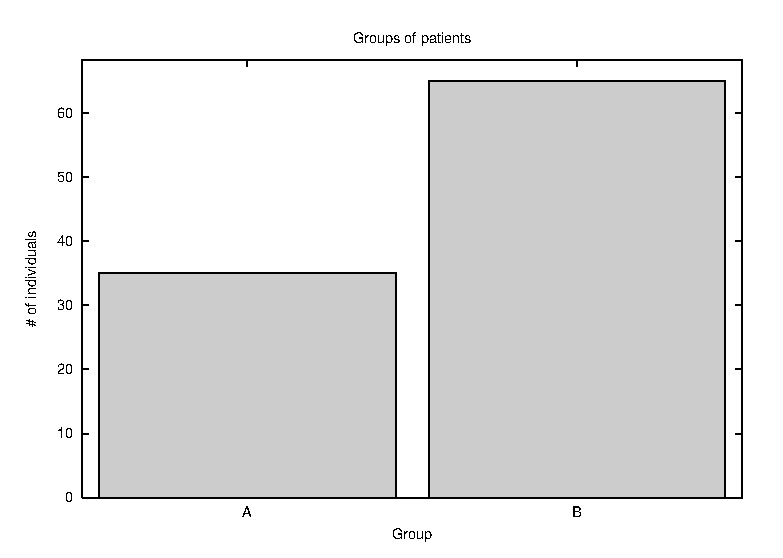
\includegraphics[scale=1.0]{barsplot1.eps} \\
\emph{a)} \\ 
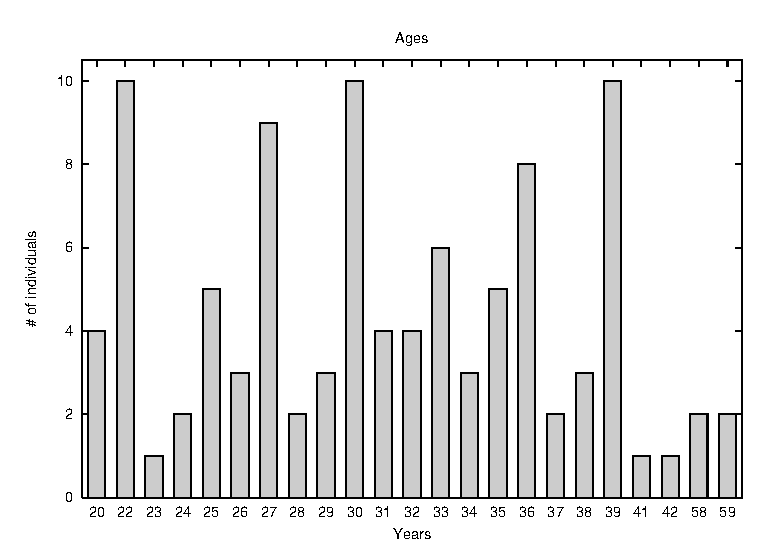
\includegraphics[scale=1.0]{barsplot2.eps} \\
\emph{b)} \\
\caption{Gr'aficos de barras: \emph{a)} de variable categ'orica; \emph{b)} de variable num'erica discreta.}
\label{fig5}
\end{center}
\end{figure}


\item[boxplot(data, options)] Esta funci'on dibuja diagramas de cajas. El argumento \verb|data| puede ser una lista, lo cual no es de gran inter'es, puesto que estos diagramas se utilizan principalmente para comparar muestras diferentes, o una matriz, de forma que sea posible comparar dos o m'as componentes de una variable estad'istica multivariante. Pero tambi'en est'a permitido que \verb|data| sea una lista de muestras con tama~nos muestrales diferentes, de hecho, esta es la 'unica funci'on del paquete \verb|descriptive.mac| que permite este tipo de estructura de datos. V'ease ejemplo m'as abajo.

\begin{enumerate}
\item \verb|'outpudev|, por defecto \verb|"x"|, indica el dispositivo de salida; valores aceptados son \verb|"x"|, \verb|"eps"| y \verb|"png"|, para la pantalla y los formatos postscript y png, respectivamente.
\item \verb|'maintitle|, por defecto \verb|""|, es el t'itulo principal entre comillas dobles.
\item \verb|'axisnames|, por defecto \verb|["sample", "y"]|,  es una lista con los nombres para los ejes $x$ e $y$.
\item \verb|'picturescales|, por defecto \verb|[1.0, 1.0]|, factores de escala para el tama~no del gr'afico.
\end{enumerate}

Las salidas de estos dos ejemplos est'an en la Figura~\ref{fig6}. Recu'erdese que cada caja se construye con los valores extremos y los cuartiles de la muestra.
\begin{verbatim}
(%i19) boxplot(s2,'outputdev="eps",
               'maintitle="Velocidad del viento en nudos",
               'axisnames=["Estaciones",""])$
(%i20) boxplot([[6,4,6,2,4,8,6,4,6,4,3,2],
               [8,10,7,9,12,8,10],
               [16,13,17,12,11,18,13,18,14,12]],
             'outputdev="eps")$
\end{verbatim}


\begin{figure}
\begin{center}
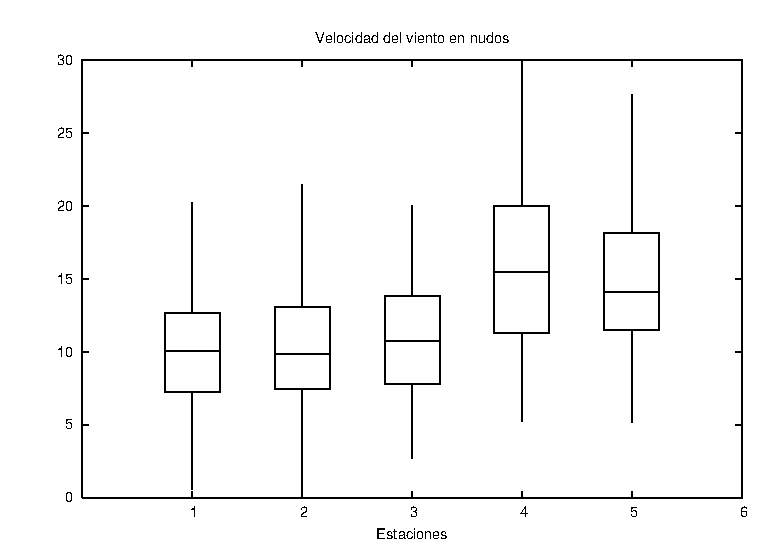
\includegraphics[scale=1.0]{boxplot1.eps} \\
\emph{a)} \\ 
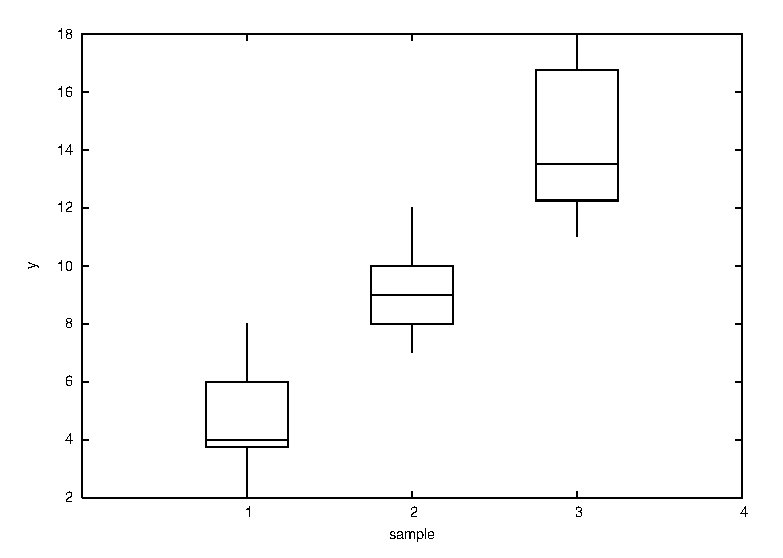
\includegraphics[scale=1.0]{boxplot2.eps} \\
\emph{b)} \\
\caption{Diagramas de cajas: \emph{a)} datos meteorol'ogicos; \emph{b)} tres muestras de diferente tama~no.}
\label{fig6}
\end{center}
\end{figure}


\end{description}


\bibliographystyle{plain}

\begin{thebibliography}{10}

\bibitem{hasl}
Haslett, J., Raftery, A. E. (1989) \emph{Space-time Modelling with
   Long-memory Dependence: Assessing Ireland's Wind Power Resource
   (with Discussion)}. Applied Statistics \textbf{38}, 1--50.

\bibitem{hynd}
Hyndman, R. J., Fan, Y. (1996) \emph{Sample quantiles in statistical
     packages}. American Statistician, \textbf{50}, 361--365.

\bibitem{john}
Johnson, A.J., Wichern, D.W. (1998) \emph{Applied Multivariate Statistical
      Analysis}. Prentice Hall.

\bibitem{pena}
Pe\~{n}a, D. (2002) \emph{An\'alisis de datos multivariantes}. McGraw-Hill, Madrid.

\bibitem{rios}
R\'{\i}os, S. (1985) \emph{M\'etodos estad\'isticos}. Ed. del Castillo, Madrid.


\end{thebibliography}

\end{document}

